\documentclass{article}
\usepackage[round]{natbib}
\usepackage{amsmath,amssymb,amsfonts, bbm}%
\usepackage{geometry}%
\usepackage{color}
\usepackage{graphicx}
\usepackage{authblk}
\usepackage{nameref}
\usepackage[right]{lineno}
\usepackage{subcaption}
\usepackage{tikz}
\usepackage{placeins}

\newcommand{\tsinfer}[0]{\texttt{tsinfer}}
\newcommand{\kwarg}[0]{\texttt{KwARG}}
\newcommand{\argweaver}[0]{\texttt{ARGweaver}}
\newcommand{\argweaverD}[0]{\texttt{ARGweaver-D}}
\newcommand{\relate}[0]{\texttt{Relate}}
\newcommand{\espalier}[0]{\texttt{Espalier}}
\newcommand{\arbores}[0]{\texttt{Arbores}}
\newcommand{\tskit}[0]{\texttt{tskit}}

% Bold the 'Figure #' in the caption and separate it from the title/caption with a period
% Captions will be left justified
\usepackage[aboveskip=1pt,labelfont=bf,labelsep=period,justification=raggedright,singlelinecheck=off]{caption}
\renewcommand{\figurename}{Fig}

% deal with supplementary items
\newcommand{\supplementarysection}{%
  \setcounter{figure}{0}% Reset figure counter
  \let\oldthefigure\thefigure% Capture figure numbering scheme
  \renewcommand{\thefigure}{S\oldthefigure}% Prefix figure number with S
  \section{Supplementary section}% Set supplementary section
}

\begin{document}

\linenumbers
\title{Computing likelihoods under the SMC for a general class of ARGs.}

% First authors
\author[1, $\dagger$]{Gertjan Bisschop}

% Middle Authors
\author[2]{Alison Etheridge}
\author[3]{Peter Ralph}

% last author
\author[1]{Jerome Kelleher}
\affil[$\dagger$]{Denotes corresponding author}

\maketitle

\affil[1]{Big Data Institute, Li Ka Shing Centre for Health Information and Discovery, University of Oxford, OX3 7LF, UK}
\affil[2]{Department of Statistics, University of Oxford, OX1 3LB, UK}
\affil[3]{University of Oregon, USA}

\section{Abstract}
This means there currently is no way to connect the output of the diverse 
range of ARG inference methods back 
to a model that would allow us to perform a probabilistic exploration of the 
ARG space around the point estimate, or likelihood-based inference

\section{Introduction}

[TL:DR] Structure the introduction around this great point from Wong et al.:
Note that it is important to distinguish here between structures and models: 
whether an inference method is based on 
heuristics or a rigorous mathematical model is orthogonal to the level 
of detail provided in its estimate. One could heuristically estimate a 
fully precise ARG, or statistically sample a partial, approximate ARG under 
a model such as the coalescent.


\subsection{ARGs are awesome, or general intro about approximations}
% approximation: level of detail
* [Importance of ARGs: ARGs as object of theoretical reasoning vs what can be known]\\
* [difference between precision/detail and accuracy. High precision can 
give a false sense of certainty in the provided estimate]. 

In population genetics, the questions we try to answer are generally 
about the unobserved processes that gave rise to the genetic variation 
we can observe given a set of samples. 
The coalescent with recombination 
Kingman, 1982a,b; Tajima, 1983; Hudson, 1983) is generally used as 
the generative model that allows us to understand the genealogy 
underlying a particular sampleset. 
Datastructure that captures it: ARG.
For a very long time people have assumed that what is meant by an ARG is the 
fully specified genealogical history  
where all events are uniquely positioned both in time
and along the genome. [However see Wong et al. 2023]. 
% say something about the difficulty of precise ARG inference (see more scalable ARG inference later on).

Although ARG, ...,
something about the level of detail.
% easy by which the CwR can be used to simulate is not matched by the usability of the model for inference

\subsection{approximations have driven the rate of progress in inference}

Instead, approximations of the coalescence with recombination (CwR) have  
driven our ability to perform statistical genomic inference. Two approximations 
in particular have proven to be instrumental [...]. Tightly linked to their 
ability to reformulate these inference problems as hidden markov Models (HMM) 
and use the well-known efficient HMM-algorithms. 
Both: 1/ Left to right, and 2/ discetization 
of state space by emumerating tree topologies and/or discretising time.\\

To improve the ability to simulate the CwR, McVean and Cardin 
provided an approximation of the CwR that is both Markovian backwards in time 
as well as left-to-right along the genome \citep{mcvean_2005_approximating}. 
By sacrificing precision on our ability to capture long range linkage 
information, the sequentially Markovian coalescent (SMC) 
became the engine of many powerful inference methods [PSMC]. 
A later improvement, the SMC', closed the gap between the SMC and the 
CwR even further.

A second key approximation is not a generative model, instead the 
copying model \citep{li_2003_modeling} was specifically designed to 
generate CwR-like patterns. 
Rather than providing a mathematical description of the genealogies 
underlying the observed data it pragmatically describes the relationship 
of a single genome to a larger set of samples as the result of an 
incomplete copying process. This heuristic approach has been successfully 
applied for demographic inference [and other things: ADD] 
\citep{sheehan_2013_estimating, steinrucken_2018}.

Both approaches have further formed the basis of the recent advancements in 
scalable ARG inference methods [references]. 
First real breakthrough, ARGweaver, samples an ARG from the posterior distribution 
given the observed variational data. Although require limiting the set of 
possible node times to be compatible with HMM algorithms, the ARGs returned 
by ARGweaver are fully precise and detailed in the sense that all 
recombination events are explictly inferred. 
This is where the real big difference lies with all other scalable methods. 
Although all different, all these methods share the fact that the ARGs they infer 
are approximate structures. The ARGs they infer have varying degrees of detail



\subsection{Recent progress in ARGs through approximate structures}

% bring nuance in the distinction between detail and approximation

% heuristic methods guided by coalescent principles (Li and Stephens)


These methods
have raised the realistic prospect of ARG-based analysis becoming a standard 
part of the population and statistical genetics toolkit.

% what is an approximate structure: implicit recombination, polytomies or not, ...
They lack the full detail: implicit recombination, ...
In particular, recombination is dealt with implicitly. Recombination events are 
not directly inferred and thus not dated. Tree topology changes from one local 
tree to the next without explicit inference of the one or more recombination 
events required to explain the inferred tree transition.

Note that approximate structure need not be an issue, the fully precise and detailed 
ARG can never be known. Instead, the main question is how to connect these 
approximate structures to the existing generative models.

\subsection{The Big problem: how do you connect such approximate structures to a generative model} 

% Existing formalisms assume that an ARG is known in full detail
These recent developments have also meant however that
we are now using the term ARG for a varying range of approximate structures 
as generated by these different inference methods \citep{wong_a-general_2023}. 
Besides not having a unified output format, the degree of completeness 
in which genetic inheritance from ancestors to 
descendants is documented by each of these methods varies extensively.
This has complicated the ability to connect the output of this diverse range of 
ARG inference methods to a model-based deescription that would allow us to perform  
probabilistic exploration of the ARG space around the point estimate, 
or likelihood-based inference (that does not just consider individual marginal trees).


\subsection{what we will do}

Here, the idea is to use the backwards-in-time formulation of the SMC to 
compute likelihoods for for \textit{any} inferred ARG 
by integrating out the time to recombination.
The application of the SMC in a way that resonates more 
with the true direction of flow of genetic information 
results in a concrete way to formulate an algorithm 
that is \textit{general} in the sense that it can deal with the various levels of 
completeness that characterise the current state of the field of ARG reconstruction.


\section{Methods and Results}
\subsection{SMC backwards-in-time}\label{par:description}

Formulated backwards-in-time, the SMC \citep{mcvean_approximating_2005} only requires a 
simple modification to the 
coalescent with recombination. By only considering those pairs of 
lineages that share 
genomic intervals with ancestral material, as eligible for coalescence, we obtain the 
sequential Markovian structure along the chromosome.\\

More formally, and following the notation of \citet{mcvean_approximating_2005}, at any 
point in time, the process can be described by $L(t)$, the set of labeled lineages 
extant at time $t$ each represented by a union of ordered non-overlapping half open 
intervals detailing the ancestral material 
carried by that lineage $X_i = \{[x_{i0}, y_{i0}), \dotsc, [x_{im}, y_{im})\}$.
$L(0)$ consists of $n$ sampled lineages, labelled $0$ to $n-1$, each represented by a 
single interval spanning the entire genome.
Backwards in time the process evolves by a succession of coalescence and recombination 
events until each segment of ancestral material is only present in one lineage. 
The waiting time to next event is determined by these two competing processes 
with exponentially distributed waiting times as outlined below.\\

Recombination is described by a Poisson process of rate $r$ per unit of length and time. 
A recombination to the 
left of $x$ with $x>x_{i0}$ and $x<y_{im}$ splits a lineage $i$ into two new, uniquely 
labelled lineages. \\ % old lineage is removed from L, two new lineages are added

Any two \emph{overlapping} lineages coalesce at rate $\lambda = 1/(2N_e)$ in the case
of a diploid population of constant size. The newly formed lineage acquires the 
union of both ordered intervals. % L is updated accordingly
Although coalescence is reciprocal, here we'll define a strict total order 
(see \ref{par:liks}) on 
all lineages in $L(t)$ based on their leftmost starting points. 
For any such strict total order on $X(t)$ and at any point in the process 
the instantaneous rate of coalescence then equals $\lambda \sum_{i \neq j} I_{ij}$.

\begin{equation} \label{def:coal}
I_{ij} = \begin{cases}
1 & X_i > X_j \wedge X_i \cap X_j \neq \emptyset \\
0 & \text{otherwise}
\end{cases}
\end{equation}

We can now define $C_i(t) = \{X_j \in L(t) | I_{ij}(t) = 1\}$ such that $|C_i(t)| = 
I_{i}(t) = \sum_{j} I_{ij}(t)$.
Because $I_{ij}$ is not reciprocal, each extant lineage has its own unique set of 
lineages $C_i(t)$ it can coalesce with. This will simplify the likelihood computations 
(see \ref{par:liks}). Note that although recombination affects $C_i(t)$ it does not 
affect $I_{i}$.\\ 

% note on the disjoint set of intervals for each lineage under the SMC
As noted by \cite{mcvean_approximating_2005}, the backwards-in-time description of the 
SMC is slightly different from the left-to-right approach in that recombination 
in non-ancestral material is possible (see fig.\ref{fig:smc-unary}). 
Although this does not affect the distribution 
of marginal genealogies, it does mean that not all lineages in $L$ can be represented 
by a single interval. More precisely, all lineages will be associated with 
a single interval up to the point where one section of the 
genome has reached its most recent common ancestor but the neighbouring parts have not.

\subsection{Recording an ARG} \label{par:recording}

The process described in the previous paragraph details the transitions of the 
set of labeled lineages $L$ through time. An Ancestral Recombination Graph 
$\mathcal{G} = (N, E)$ capturing the various inheritance paths along the genome 
is obtained by registering an edge represented by a tuple $(c, p, X_{cp})$ 
whenever a lineage $c$, associated with a disjoint set of genomic intervals $X_c$, is 
replaced by one or two lineage(s), $p$ (and $p^{\prime}$), 
in case of a coalescence or recombination respectively.
The last element of the tuple is the extent of the edge. It is itself a  
disjoint set of intervals such that $X_{cp} \cup X_{cp^{\prime}} = X_c$. 
The set of edges $E$, containing all such tuples $(c, p, X_{cp})$, 
and $N$, the set of nodes representing all genomes in the ARG, together
define this data structure.\\

The ARG as described here records the impact of every possible event along each 
inheritance path in full detail. Fig.\ref{fig:smc-unary} shows one such possible 
ARG generated represented 
as both a graph (top) as well as a series of local trees (bottom). 
Note that both structures represent the same information. 
Crucial for the equivalence between both representations is the presence of
nodes that (locally) only have a single child along one or more local 
trees. Not all of these (locally) unary nodes are 
(blue, fig.\ref{fig:smc-unary}) recombinant nodes. By recording edges along 
the full extent of each lineage, coalescing nodes can be locally unary 
along particular genome intervals. Furthermore, the unary nodes enable 
us to uniquely identify all lineages that were hit by a recombination 
event, even when we simplify the ARG by removing all 
(blue, fig.\ref{fig:smc-unary}) recombinant nodes. 
In the absence of recombination nodes, a recombination can be observed 
easily enough on the local trees as a change in parent going from 
one tree to the next. This simplification step 
does mean however that we lose precise time information on the 
recombination events. Yet we can constrain the uncertainty to 
within a window defined by the age of the child node $c$ associated 
with that lineage and the minimum age of the parents of the 
edges connecting to $c$. This in turn is easier to visualise using the 
graph representation (blue shaded area, fig.\ref{fig:smc-unary}).\\

ARG simplification is thus linked to the presence of unary nodes in 
the local trees and simultaneously touches upon the question of what is 
knowable. Many ARG reconstruction methods return a data structure that 
is in essence a series of local tries [REFs]. 
As highlighted, this does not need to be a contradiction. 
All ARGs can be represented as a series of local trees \citep{wong-2023}.
The important question is therefore is however about the extent by which any 
ARG reconstruction methods incorporates the available information 
on how nodes persist across these local trees.\\ 

[TO DO] give a good explanation (using the represented haplotypes 
in fig. \ref{fig:smc-unary}) on why these methods can infer the extent 
of coalescing lineages.
Currently, the following methods 
return the full this information by default as part of their ARG reconstruction algorithm: 
\argweaver \citep{rasmussen_genome-wide_2014} 
\tsinfer \citep{kelleher_inferring_2019}, 
\kwarg \citep{ignatieva_kwarg_2021}.\\


[TO DO]: impact of unary nodes on reasoning about the SMC in a left-to-right sense.\\

In the next paragraph we will derive an expression to compute the 
likelihood for an ARG under the SMC for which we have no information on the 
time to any of the recombination events. We will then detail an algorithm 
that allows us to compute this value given an ARG 
represented as a series of local trees. To do this we will rely on the unary nodes 
to identify each lineage involved in a recombination event 
as described in this section.


\begin{figure}[!ht]
\centering
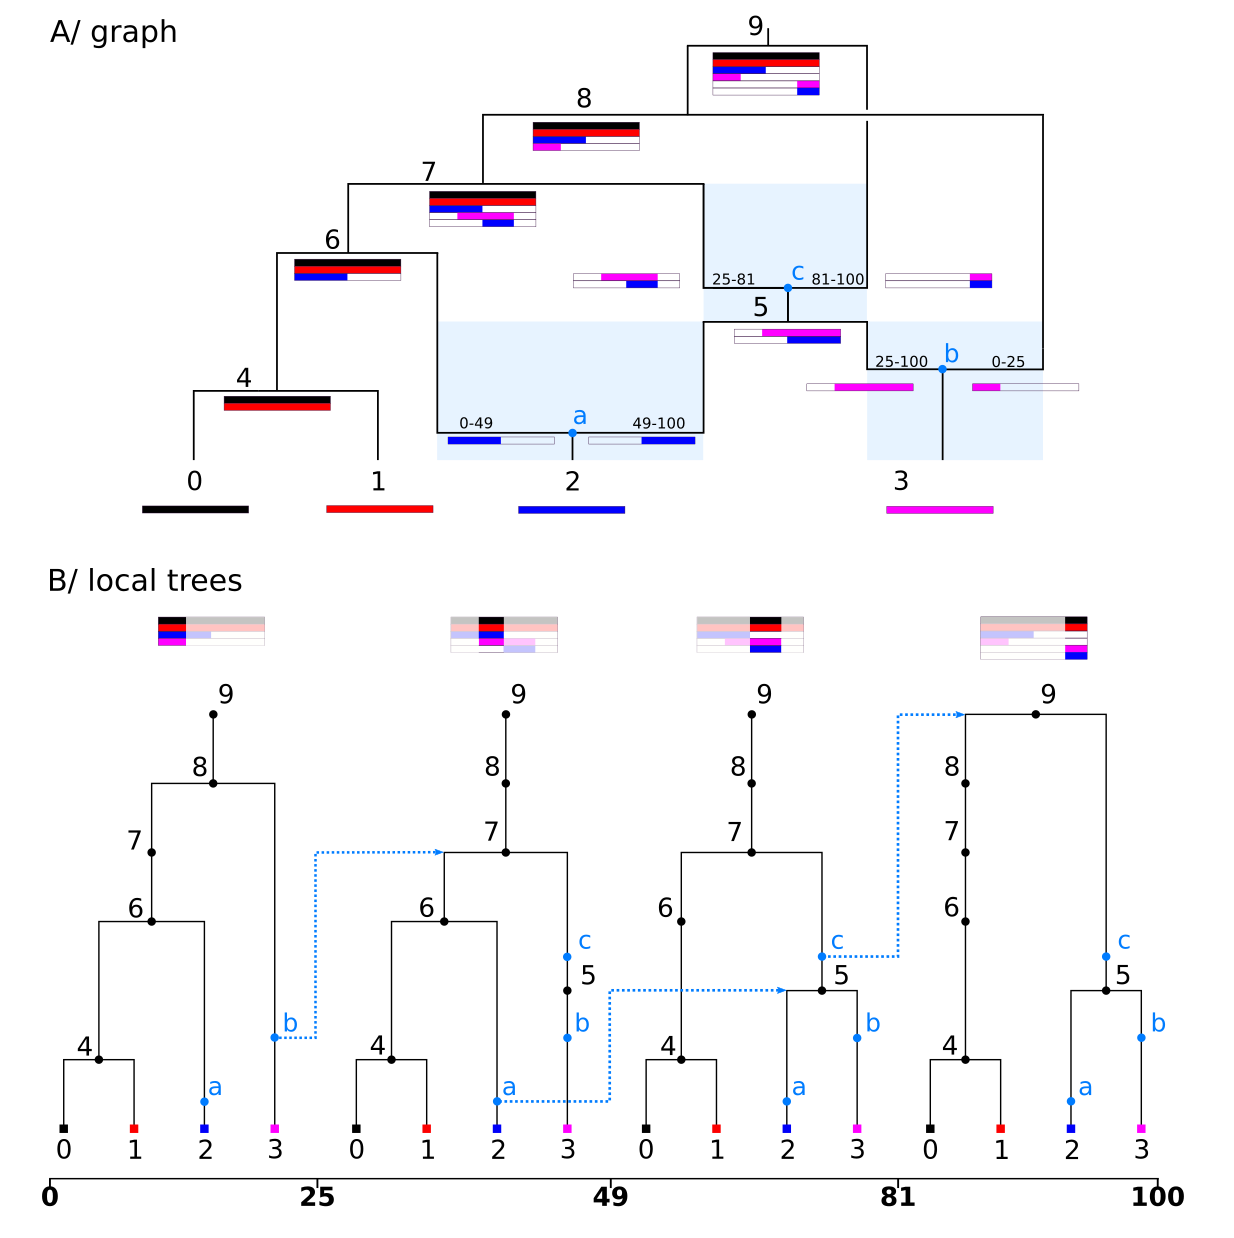
\includegraphics[width=\textwidth]{figures/smc_custom_2rows_area.png}
\caption{ARG generated under the SMC and its representation as a 
series of local trees (bottom). To ensure the one-to-one correspondance 
between both representations a node is recorded for each local tree whenever 
a node is encoundered along its ancestry path in the graph representation. 
This results in nodes that (locally) have only a single child, and are therefore 
(locally) unary. Blue (unary) nodes represent recombinant nodes. 
The blue arrows shows the familiar left-to-right logic of the SMC whereby 
the floating lineage coalesces randomly
with a the remaining portion of the local tree following recombination.
Note how the presence of the unary node on a local tree is 
indicative of either a past (to the left of the local tree) 
or future (to the right) coalescence event. 
Both ARG representations can be simplified by removing the recombinant nodes. 
In that case the information we have on the time to each of these events is 
limited to the windows (blue shaded array) delimited by by the age of 
the child node $c$ associated with that lineage and the minimum age of 
the parents of the edges connecting to $c$. 
 [TO DO: wanted to use the 
added in haplotype information to explain why we can actually infer the 
extent of each lineage, and thus create unary nodes in the first place.]
}
\label{fig:smc-unary}
\end{figure}



\subsection{Calculating likelihoods} \label{par:liks}

Retracing the ARG backwards in time, each coalescence event is associated with two child 
lineages, $c$ and $d$, and a single parent, $p$. By defining $C_i(t)$ asymmetrically, 
the history of each these two child lineages can be considered independently without 
risking to double count any of the coalescence events. The likelihood of 
observing the edge $(c, p, X_{cp})$ can thus be considered independently from 
the likelihood of all other edges, and in particular from the likelihood 
of $(d, p, X_{dp})$.\\

% extends from here means min(X_{cp})=x, max(X_{cp})=y
% improve this description here
Assuming $(c, p, X_{cp})$ extends from $x$ to $y$ along the genome and $t_i$ 
indicates the age of 
node $i$ in the ARG, then the probability of not observing a recombination across the 
entire area (span x depth) of this edge is 

% full extent of segment
\begin{equation}\label{eq:span}
A_{(c, p)}(\theta) = e^{-r (y-x)(t_p - t_{c})}
\end{equation}
% also x and y not necessarily equal to x_{c_{1}0} and y_{c_{1}m}.

What's left to compute the likelihood of the focal edge, is to take into account 
all events associated with $x$, 
the leftmost coordinate of $(c, p, X_{cp})$. 
This is either only the 
coalescence event involving 
$c$ and $d$. In that case $x=x_{c0}$ and $c$ did not coalesce until $t_p$. 
Alternatively, $x$ can be a new recombination break point that 
occurred on the lineage represented by $c$ at some time $s$ between $t_{c}$ 
and $\min(t_p, t_{p^{\prime}})$, where $p^{\prime}$ is the parent of the 
edge $(c, p^{\prime}, X_{cp^{\prime}})$ ending at $x$. The new lineage formed 
by the recombination event and starting at $x$ can be given a temporary label 
$c_s$. In both cases, the cumulative hazard of a lineage $a$ coalescing 
between time $s$ and $t$ is given by $F(c, s, t) = \int_{s}^{t} I_{c}(u)du$ 
such that:

\begin{equation}\label{eq:depth}
B_{(c, p)}(\theta) = \begin{cases}
e^{-\lambda F(c, t_c, t_p)} \lambda^{I_{cd}(t_p)} & x=x_{c0} \\
\int_{t_c}^{t_{p} \wedge t_{p^{\prime}}} r e^{-rs} e^{-\lambda F(c_s, s, t_{p})} ds \lambda^{I_{c_{s}d}(t_p)} & x=x_{c_{s}0}>x_{c0} \\
\end{cases}
\end{equation}

Here, the (second) exponential term gives the probability of not observing a 
coalescence event before $t_p$. In case of a recombination, $re^{-rs}$ further 
gives the probability of observing a recombination 
at time $s$ given a Poisson process along position $x$ with rate $r$. The 
time of the recombination is integrated out.
The last term gives the point probability density of the coalescence event 
that terminates the edge. The indicator function is used to resolve 
the non-reciprocal nature of coalescence events as defined in \ref{def:coal}.\\

The likelihood of ARG $\mathcal{G}$ defined by the set of edges $E$ and
given parameters $\theta$ then is

\begin{equation}\label{eq:full-lik}
\mathcal{L}(\mathcal{G}|\theta) = \prod_{(c, p) \in E} A_{(c, p)}(\theta) * B_{(c, p)}(\theta)
\end{equation}

% Does this hold for the case beyond the root of the genealogy?

[TO DO: improve this remark: when recording an ARG we do record edges in this situation,
however, msprime simulations will stop recording edges for local trees that have reached 
their local mrca.] 
Because the likelihood is computed based on edges,
and edges are no longer recorded once the local most recent common ancestor 
has been reached, we will underestimate the number of positions where 
a recombination could have occurred in case a recombination hits a 
lineage with trapped non-ancestral material (see end \ref{par:description}). 
If we assume that only a single recombination could have  
occurred, then it suffices however to provide a correction factor $g$ in equation
\ref{eq:depth}. Here $g$ represents the 
length of non-ancestral material along which a recombination would have resulted  
in the same observed local sequence of tree changes.\\


\begin{figure}[!ht] \label{fig:algo}
\centering
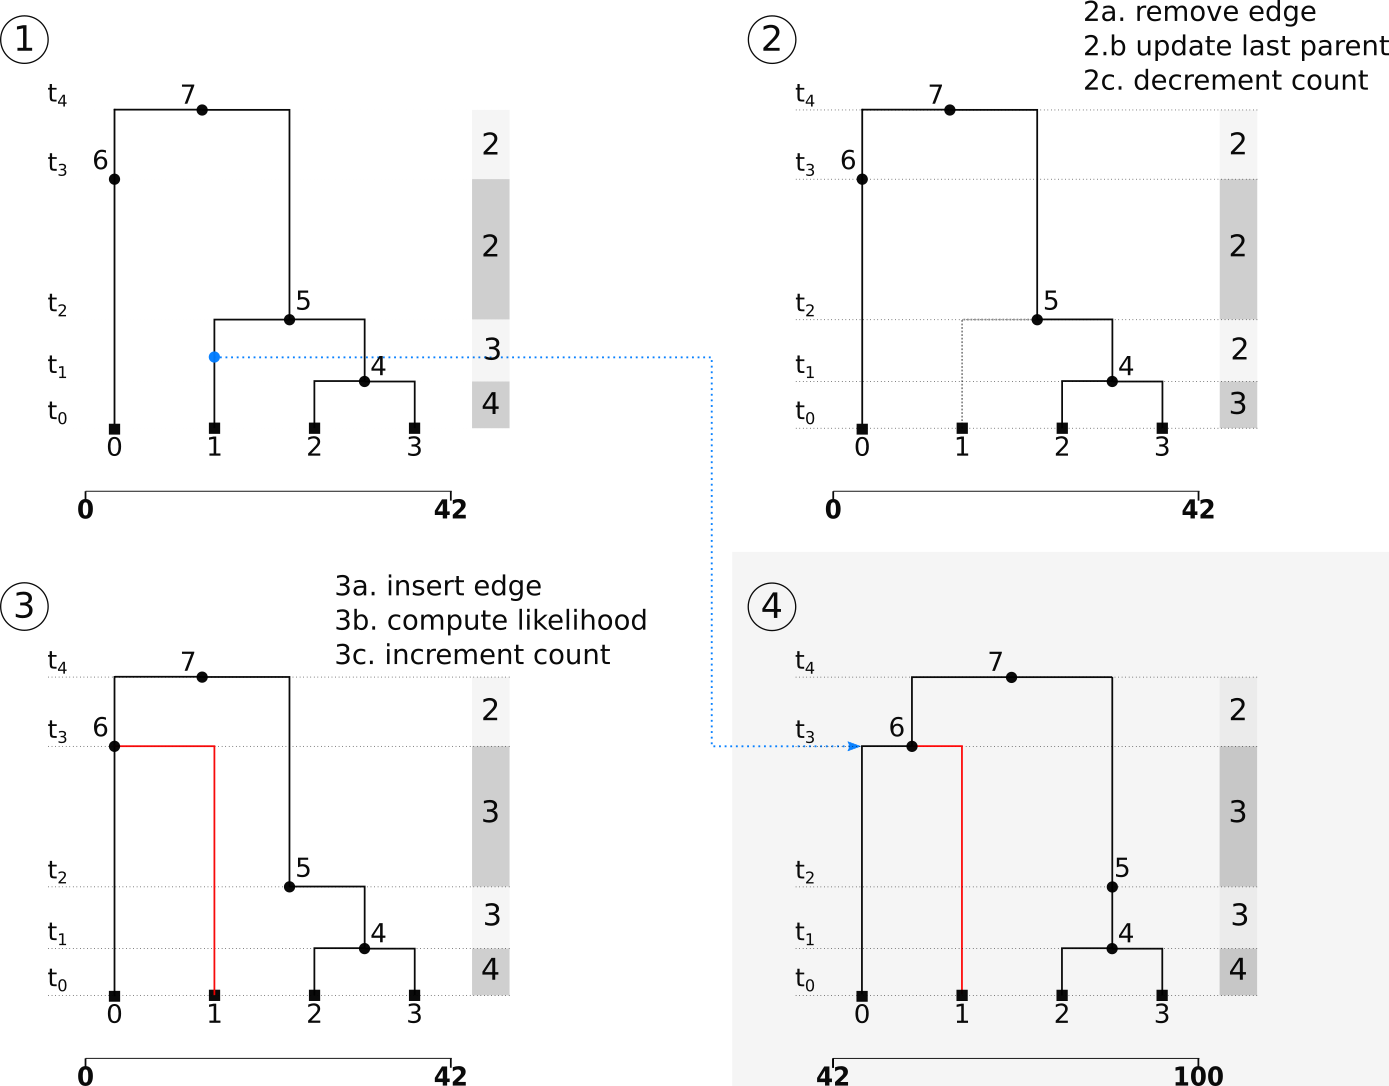
\includegraphics[width=\textwidth]{figures/ts_algo_2rows.png}
\caption{Description of algorithm: Moving along the genome we transition from  
local tree $T_1$ to the next, $T_2$ in three steps. 
Edges that do not persist in $T_2$ are 
removed first. Edges starting at the left coordinate of $T_2$ are inserted. 
After deletion or insertion of an edge the count vector $I$ is updated along the 
corresponding internode intervals. Following an insertion, and prior to updating $I$, 
the likelihood for that edge is computed as $I$ then represents the total number of 
lineages the lineage associated with this new edge can 
coalesce with. By moving along the genome in this way, each edge gets visited exactly once.}
\end{figure}

Note that we are only considering the topology and branch length information of any ARG. 
Extending this expression by adding the likelihood of observing a set of mutations 
given an ARG is straightforward.


\subsection{Tree sequence format} \label{par:algo}

Although the argument outlined in the previous paragraph is valid for any ARG, here we 
will describe how to (efficiently) extract the information required to associate a
tree sequence encoding of an ARG with a likelihood under the SMC (see fig. \ref{fig:smc-unary}).\\

Formally, we represent a tree sequence using a set of tables \citep{kelleher_efficient_2018}. 
This simple tabular representation of any ARG $\mathcal{G} = (N, E)$, can be 
augmented with additional tables with information on sequence variation
using a site and mutation table. The node table stores information on all 
haplotypes $N$ in the tree sequence. Information about how nodes relate to 
each other along the genome is defined in a tabular encoding of $E$.
Each row in this edge table constitutes a tuple \texttt{(left, right, parent, child)}.
Note that we defined the extent of any edge $\epsilon \in \mathcal{G}$ as the union of 
disjoint intervals. In the tree sequence encoding however, $\epsilon$ will be represented 
by a single entry for each contiguous interval. As remarked before, under the SMC, this 
distinction only matters beyond the root of the genealogy. The distinction between both 
types of edges will therefore not be made in the remainder of the paper.
% Although it does requires us to keep track of some additional information to avoid
% wrongfully assuming a recombination event happened.
% Similarly, the distinction between the lineage associated with an edge, and the edge 
% itself can render things very verbose.
\\

The likelihood computation as described above can be done with a single pass 
of the edge table.
The central problem however is to efficiently maintain the state $I_e(t)$, which counts 
the number of lineages (the lineage associated with) the focal edge $\epsilon$ can coalesce 
with at time $t$. 
The definition of $I_{kl}$ (\ref{def:coal}) is based on the assumption 
that we can impose a strict total order on all (overlapping) lineages based on their 
starting point. The tree sequence encoding provides us with a natural order on all lineages.  
For each local tree with left coordinate $x$, lineages associated with an edge 
starting at $x$ can only coalesce with the subset of lineages associated with one of the
edges that make up that local tree. Each of these edges will either already have 
been present in the previous local tree, or will have the same starting point $x$.
In \texttt{tskit}, the order in which edges are inserted and removed 
while moving from one tree to the next, is determined by the index 
vectors $\textbf{i}$ and $\textbf{o}$ \citep{kelleher_efficient_2016}.
The edge insertion vector $\textbf{i}$ gives the ordering of edges sorted by left 
endpoint, and among edges with the same left endpoint, sorted so that edges closer 
to the root appear later. The edge removal vector $\textbf{o}$ is similar, 
except gives the ordering of edges by right endpoint and with edges closer to the 
root appearing sooner. The variables $\texttt{i}$ and 
$\texttt{o}$ are used to keep track of our position in the edge insertion and edge removal 
indexes as we move along the tree sequence. This order imposes the 
strong ordering on all edges as required by the definition of $I_{kl}$.\\

% edge diff algorithm
The size of the subset of lineages in each internode interval each lineage 
can coalesce with can thus be maintained by keeping track of a single vector $I$ 
that is decremented or incremented as defined by
$\textbf{o}[\texttt{o}]$ and $\textbf{i}[\texttt{i}]$, 
Further keep track of a last-parent array to detect recombination events.
We can thus compute a likelihood for the tree sequence, while visiting each edge only once.

More concretely, prior to inserting an edge, $I$ represents the number of lineages 
the lineage associated with 
that edge can coalesce with. Then insert the edge and update the counts.

To transition from one tree to the next, we first iterate across the indices of all edges 
in $\textbf{o}$ from its current index up to $\texttt{o}$. For each edge in we decrement $I$ 
from index \texttt{edge.child} to \texttt{edge.parent}. We subsequently iterate across the 
edges in $\textbf{i}$ up to index $\texttt{i}$. For each new edge, we first compute the likelihood 
associated with that edge and then 
increment $I$ from \texttt{edge.child} to \texttt{edge.parent}.\\

% ADD IN RESULTS
Figure \ref{sup:fig:vs-argweaver} shows the expected near-perfect correlation 
between the coalescent prior as returned by \argweaver and the likelihood as computed here. 
We simulated 1Mb of data for 10 diploid individuals 
under the SMC using human-like parameters. 100 samples were taking from the posterior every for 
a total of 1000 MCMC iterations.
 

\subsection{Flexibility / general class of ARGs}

% slicing of the ARG
By explicitly associating a single likelihood with each edge, we can compute a likelihood 
under the SMC for any valid tree sequence. The \tskit library provides a whole range  
of subsetting operations on tree sequences allowing us to slice the ARG in time and/or space, 
as well as reduce the number of tracked samples. 
Any such subset of the tree sequence is itself a valid tree sequence 
that can again be used to compute a likelihood with. Our approach therefore strenghtens 
the inherent ability of ARGs to provide us with temporal 
resolution on the inferred genealogical history of a sample. 
We can further readily incorporate changes in $N_e$ and $r$, 
both in time as well as along the genome by respectively adding intervals to $I$ 
or by splitting edges when/wherever the parameter set changes.
[NOTE: these options have already been implemented in the current implementation]

Although we rely heavily on unary nodes to provide us with the necessary 
information on recombination events, our algorithm only implicitly assumes their presence.
The algorithm can therefore also accomodate for 
those inferred ARGs that lack unary nodes (e.g.\ \relate). 
Without unary nodes though, our algorithm will detect a recombination event along 
both coalescing lineages in case of a (sub)tree height changes along the ARG as both 
edges would switch parent nodes. This can be mitigated by limiting the number of 
'inferrable' recombination events per coalescence event to 1.

[TO DO]: improve results sections with some good viz,
We simulated 1000 ARGs under the Hudson coalescent retaining all recombination information 
and computed the corresponding likelihood using \texttt{msprime} \citep{baumdicker_efficient_2021}. 
After removing the recombination nodes the likelihoods as defined here were computed both with and 
without the unary nodes. Figure \ref{sup:fig:vs-hudson} shows that the proportion of variation 
explained is higher when the unary nodes are retained.

% polytomies
[TO DO: polytomies] The above algorithm treats each edge independently which implies 
we can deal with polytomies.
[TO DO: discuss, what if the identity of internal nodes is not preserved across trees]
[TO DO: recombination]: We do not *explicitly* assume a single recombination breakpoint to have 
occurred at each breakpoint.
[TO DO:] On a similar note and more general: we can compute the likelihood for any 
valid tree sequence, however, future work to verify to what extent/in which scenarios 
this is actually helpful.
 
\section{Discussion}

Here, we have introduced a scalable algorithm to compute likelihoods 
under the SMC for a general class of ARGs. By formulating the SMC backwards in time 
we were able to associate a single likelihood value with each edge in the ARG. 
The compatibility of the algorithm with the \texttt{tskit} library allows us to 
exploit its associated efficiencies both for the current work and its future 
applications. This work will contribute significantly 
to ARG-based analysis becoming a standard part of the population 
and statistical genetics toolkit. 
In particular, we see three main applications for the work presented here. 
Firstly, the ability to associate inferred ARGs with a likelihood given a demographic 
model and an associated set of parameters will help bridge the gap between the tremendous recent 
advances in ARG inference and the current state of the art statistical inference of 
past demography. 
Secondly, inferred ARGs can be used as a good starting point for a future MCMC sampler.
Thirdly, hybrid ARG-inference methods that combine the best of both 
heuristic and model-based inference approaches are now possible.
Finally, using a model we can quantify the uncertainty inherently associated 
with ARG-reconstruction.

% 1/ statistical inference
Currently most/all ARG-based inference methods base their analysis on marginal 
trees \citep{hejase_2022} [TO DO: add more refs]. The theory and associated algorithm 
provided here can function as a building block of 
 
$N_e$-changes as well as multiple populations and migration can be readily incorporated 
in the current algorithm.\\

% 2/ great starting point for MCMC
Any inferred ARG can be used a good starting point 
for a future MCMC-sampler. This potentially implies a massive runtime reduction by 
reducing the necessary burn-in period. Furthermore, by integrating out the exact time 
to the recombination event we further restrict the size of the ARG space that needs to 
be explored. This MCMC-sampler would again rely on the tree sequence data structure to 
efficiently generate and evaluate any new proposal (see \citep{mahmoudi_bayesian_2022}).
[TO DO:] 

% 3/ hybrid ARG-inference: scalability + bringing ARG down from pedigree dominated phase
Hybrid backwards-in-time simulations that combine Wright-Fisher dynamics in the 
very recent past and coalescent simulations for the remaining time are a tried and tested 
approach \citep{bhaskar_distortion_2014, nelson_accounting_2020} to enable large scale 
simulations while avoiding the documented biases of the coalescent relative to the 
Wright-Fisher model \citep{bhaskar_distortion_2014, wakeley_gene_2012}. The same approach 
could be used for ARG-inference where one can rely on a heuristic inference method for 
the recent past, while using a model-based approach beyond that cutoff point.\\

% 4/ quantifying uncertainty [unfinished]:
Both of these future directions tie in with the desired ability of any ARG-related method to 
quantify the uncertainty associated with 



This will in particular enable us to deal with those 
parts in both time and along the genome for which we have insufficient information to confidently 
reconstruct the ARG. The presence of polytomies in ARGs inferred by \tsinfer, for example, 
represents uncertainty. Systematicallty breaking them by sampling from the coalescent rather 
then randomly would already be a major step forward. 


Quantifying uncertainty would not necessarily always have to be associated 
with sampling 
with dealing with the entire subset of all compatible genealogies. Uncertainty could also 
be quantified and passed on as metadata to a parent node representing the uncertainty 
in the interval spanned by the polytomy.
% can something similar be done for stacked recombinations?

[TO DO] Comment on accuracy. The described algorithm has been implemented in such a way that 
any valid tree sequence will result in a likelihood value. This also holds for any tree sequence 
that does not meet the assumptions. We see it as future work to determine to what extent 
particular deviations from these assumptions will affect the shape of the likelihood surface given 
a set of parameters.

% final conclusion


\section{Data availability}

All scripts and data used for this manuscript are available on https://github.com/gertjanbisschop/smc-bit-paper
An implementation of the algorithm is available on https://github.com/gertjanbisschop/runsmc.
\FloatBarrier
\bibliographystyle{plainnat}
\bibliography{paper.bib, temp.bib}

\pagebreak 

\supplementarysection
\section*{Supplementary Information}


\begin{figure}[!ht]
\centering
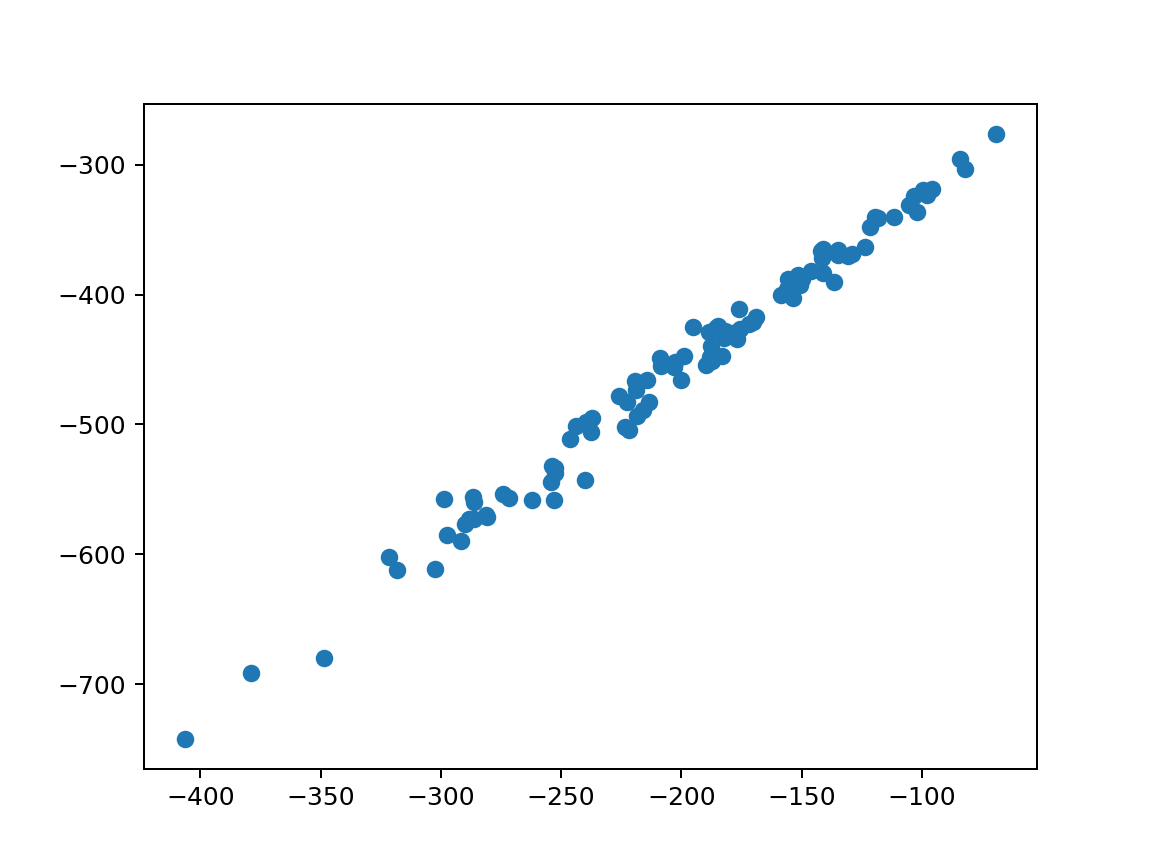
\includegraphics[width=0.75\textwidth]{figures/supplementary-figs/argweaver_vs_runsmc.png}
\caption{Simulated 10kb sequence under human-like parameters, 10 diploid samples. Inferred ARG using ARGweaver. Scatterplot is comparison of prior (discretized SMC) as reported by ARGweaver (x-axis) and likelihood as defined here (y-axis).}
 \label{sup:fig:vs-argweaver}
\end{figure}


\begin{figure}[!ht]
\centering
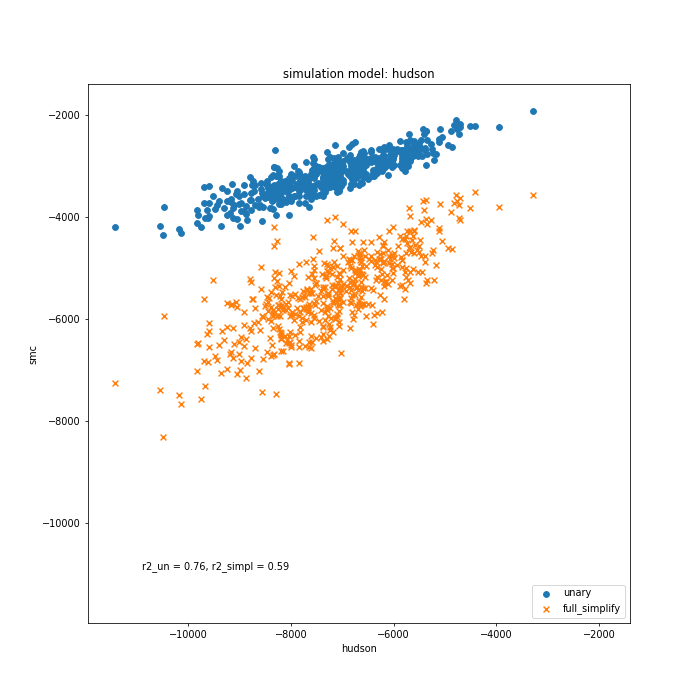
\includegraphics[width=0.75\textwidth]{figures/supplementary-figs/v_hudson_unary_simpl.png}
\caption{Compare likelihoods Hudson (full ARG) and SMC with and without unary nodes (without recombination nodes): placeholder for final figure with similar content.}
\label{sup:fig:vs-hudson}
\end{figure}


\begin{figure}[!ht]
\centering
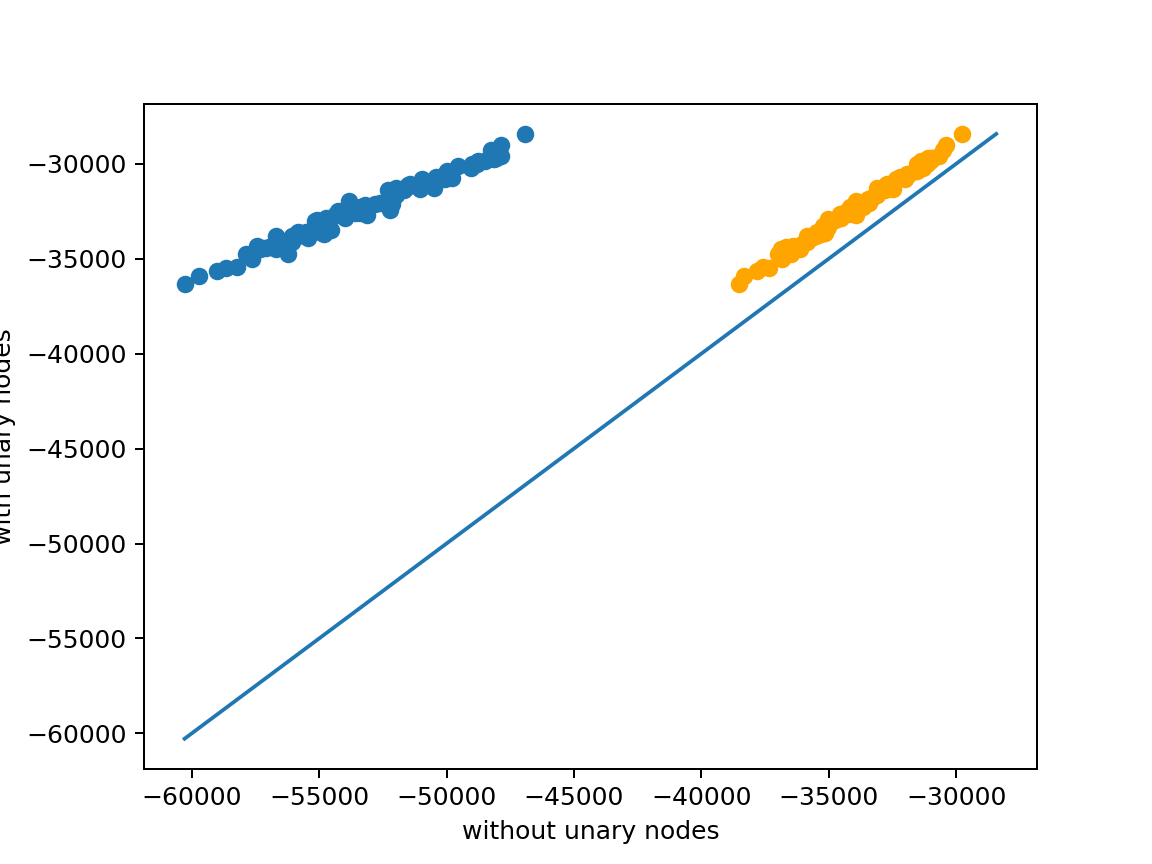
\includegraphics[width=0.75\textwidth]{figures/supplementary-figs/without_unary.png}
\caption{Simulated 1Mb of sequence under human-like parameters. Computed likelihood as defined here with unary nodes (y-axis), and without, blue dots (x-axis). By limiting the number of recombinations (to 1 event) leading up to a single coalescent node we obtain the values in orange.}
 \label{sup:fig:rec-correction}
\end{figure}

\begin{figure}[!ht]
\centering
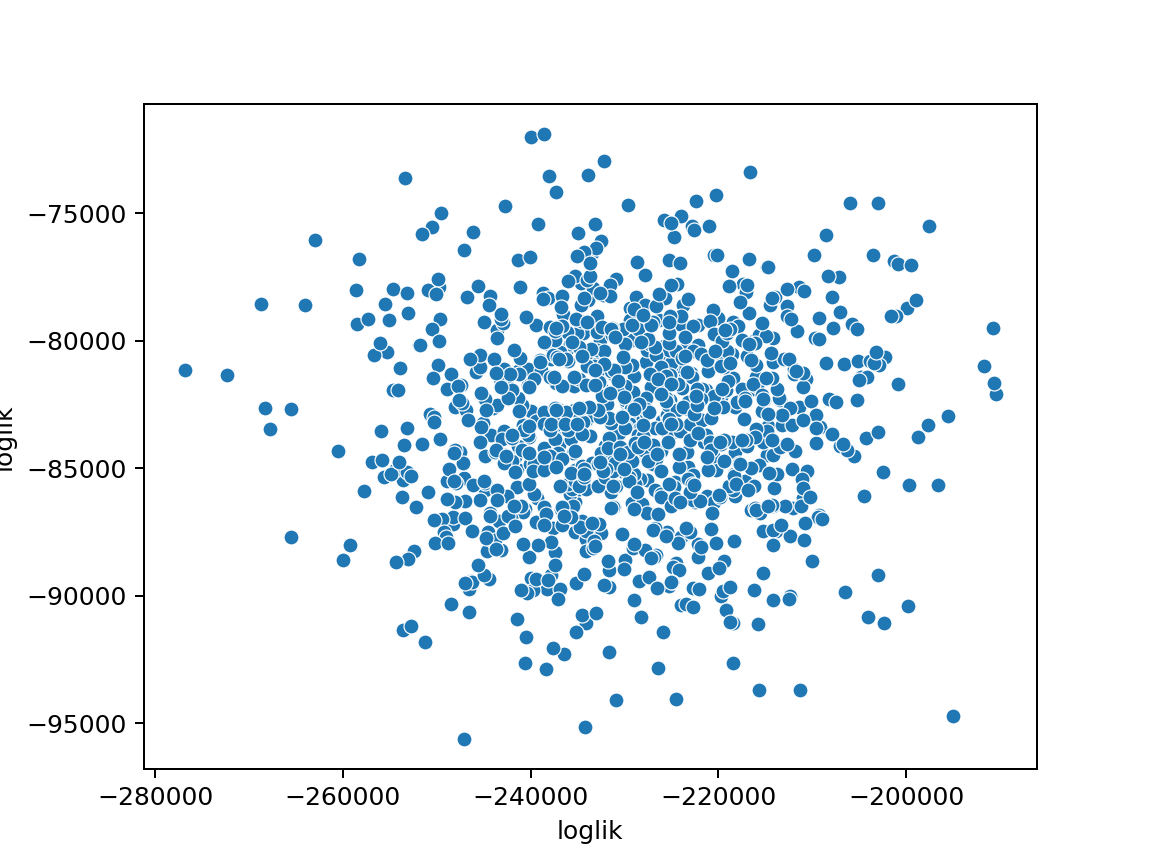
\includegraphics[width=0.75\textwidth]{figures/supplementary-figs/hudson_liks_vs_tsinfer_smc.png}
\caption{Simulated full ARG for 1Mb sequence under human-like parameters (100 diploid samples). Computed likelihood (x-axis) under Hudson. Then inferred ARG with \tsinfer following a random sprinkling of mutations and computed likelihood under SMC (y-axis)}
 \label{sup:fig:hudson-smc}
\end{figure}

\begin{figure}[!ht]
\centering
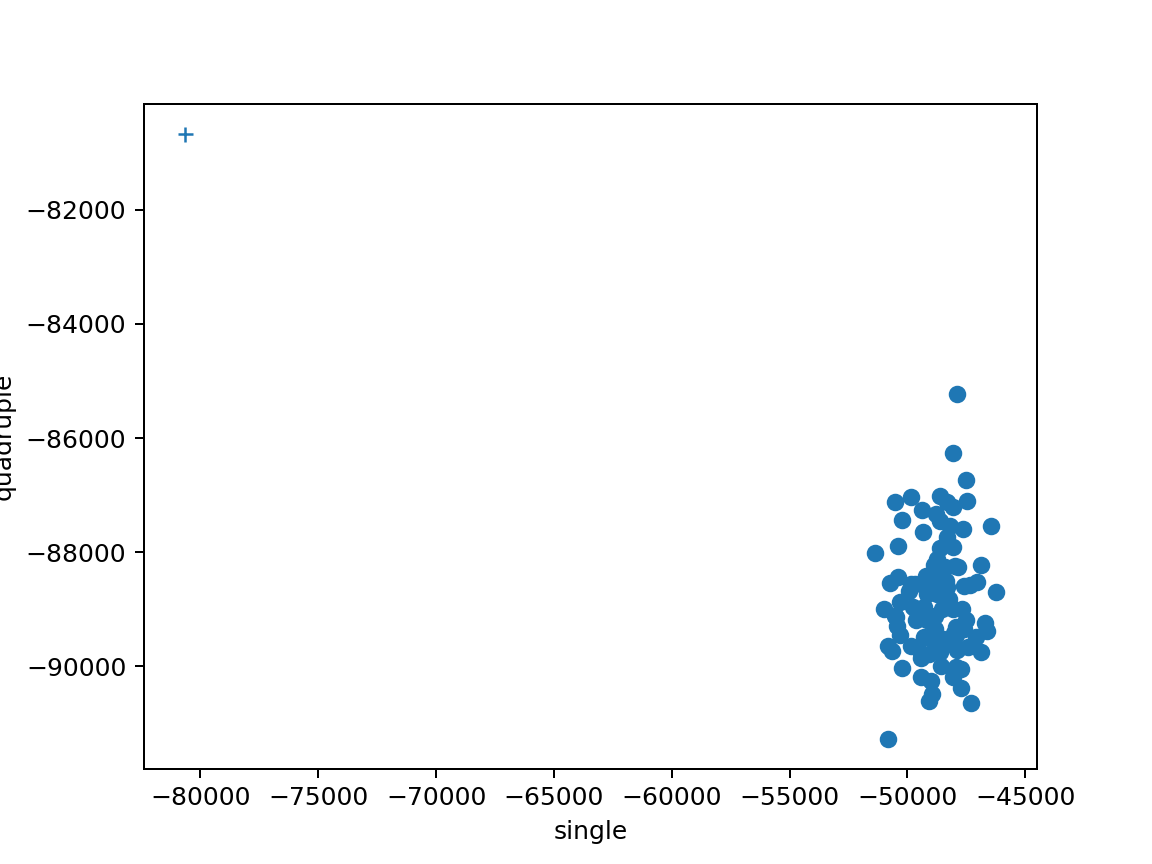
\includegraphics[width=0.75\textwidth]{figures/supplementary-figs/single_rep_human_like_1gb.png}
\caption{Single replicate from the dataset simulated above with a 100 random sprinklings of mutations. Likelihood under the SMC, mutation rate $\mu=1.25e-8$ (x-axis), and with mutation rate $4*\mu$ (y-axis). Likelihood for the full ARG under Hudson is indicated with the cross.}
 \label{sup:fig:single-tsinfer}
\end{figure}

\end{document}
